% ---------- compact preamble ----------
\documentclass[9pt,a4paper]{extarticle}
\usepackage[a4paper,margin=13mm,top=15mm,bottom=16mm,headsep=4mm,footskip=7mm]{geometry}
\usepackage[T1]{fontenc}\usepackage[utf8]{inputenc}
\usepackage{newtxtext}  % Times, as in the ICML template
\usepackage[scaled=0.82]{sourcecodepro}
\usepackage{microtype}
\setlength{\emergencystretch}{2em} % let narrow columns wrap long tokens instead of overflowing
\usepackage{amsmath,amssymb}
\usepackage{newtxmath}   % matching Times math
\usepackage[table,dvipsnames]{xcolor}
\usepackage{booktabs,multicol,tabularx,makecell,array,longtable}
\renewcommand*\setemergencystretch[2]{\emergencystretch 2em} % multicol otherwise resets it to 4pt per column
\usepackage{graphicx}
\usepackage{enumitem}
\usepackage{titlesec}
\usepackage{fancyhdr}
\usepackage{caption}
\usepackage{tcolorbox}\tcbuselibrary{skins,breakable}
\usepackage{tikz}\usetikzlibrary{positioning,arrows.meta,shapes,calc,fit,backgrounds}
\usepackage{pgfplots}\pgfplotsset{compat=1.18}
\usepackage{fontawesome5}
\usepackage{ragged2e}
\usepackage{CJKutf8}\newcommand{\cjk}[1]{\begin{CJK*}{UTF8}{gbsn}#1\end{CJK*}}
\usepackage[colorlinks,linkcolor=linkc,urlcolor=linkc,citecolor=linkc]{hyperref}

% ---------- palette (dataviz reference palette) ----------
\definecolor{s1}{HTML}{2a78d6}\definecolor{s2}{HTML}{eb6834}\definecolor{s3}{HTML}{1baf7a}
\definecolor{s4}{HTML}{eda100}\definecolor{s5}{HTML}{e87ba4}\definecolor{s6}{HTML}{008300}
\definecolor{s7}{HTML}{6250d6}\definecolor{s8}{HTML}{e34948}
\definecolor{critical}{HTML}{d03b3b}\definecolor{good}{HTML}{0ca30c}\definecolor{warning}{HTML}{fab219}
\definecolor{ink}{HTML}{0b0b0b}\definecolor{ink2}{HTML}{52514e}\definecolor{ink3}{HTML}{8a8984}
\definecolor{surface}{HTML}{f6f5f2}\definecolor{rule}{HTML}{d9d8d2}\definecolor{linkc}{HTML}{1c5cab}
\colorlet{agA}{s1}\colorlet{agB}{s2}\colorlet{agC}{s3}\colorlet{agD}{s7}
\colorlet{agE}{s5}\colorlet{agF}{s4}\colorlet{agG}{s6}\colorlet{agH}{ink3}

% ---------- typography ----------
\setlength{\parindent}{0pt}\setlength{\parskip}{2.5pt plus 1pt}
\setlength{\columnsep}{6mm}
\linespread{0.98}
\titleformat{\section}{\Large\bfseries\color{ink}}{\thesection}{0.6em}{}
\titlespacing*{\section}{0pt}{9pt plus 2pt}{4pt}
\titleformat{\subsection}{\large\bfseries\color{ink}}{\thesubsection}{0.6em}{}
\titlespacing*{\subsection}{0pt}{7pt plus 2pt}{3pt}
\titleformat{\subsubsection}{\normalsize\bfseries\color{ink2}}{\thesubsubsection}{0.5em}{}
\titlespacing*{\subsubsection}{0pt}{5pt plus 1pt}{2pt}
\titleformat{\paragraph}[runin]{\bfseries\color{ink2}}{}{0pt}{}[.\ ]
\titlespacing*{\paragraph}{0pt}{3pt}{0.5em}
\setlist{nosep,leftmargin=1.2em,itemsep=1pt}
\captionsetup{font={small,color=ink2},labelfont=bf,skip=3pt}
\renewcommand{\arraystretch}{1.08}
\makeatletter\setlength{\@fptop}{0pt}\makeatother
\pagestyle{fancy}\fancyhf{}
\fancyhead[L]{\footnotesize\color{ink2}Failure-attribution datasets for LLM agents}
\fancyhead[R]{\footnotesize\color{ink2}\nouppercase{\leftmark}}
\fancyfoot[C]{\footnotesize\color{ink2}\thepage}
\renewcommand{\headrulewidth}{0.3pt}\renewcommand{\headrule}{\color{rule}\hrule width\headwidth height 0.3pt}

% ---------- helper macros ----------
\newcommand{\code}[1]{\texttt{\small\def\_{\textunderscore\allowbreak}#1}}  % underscores are break points
\newcommand{\chip}[2]{\tikz[baseline=(t.base)]\node[fill=#1!18,text=#1!60!black,rounded corners=2pt,inner xsep=3pt,inner ysep=1.5pt,font=\scriptsize\bfseries](t){#2};}
\newcommand{\okbadge}{\chip{good}{available}}
\newcommand{\gatedbadge}{\chip{warning}{gated}}
\newcommand{\nobadge}{\chip{critical}{not released}}
\newcommand{\partialbadge}{\chip{s7}{partial}}
\newcommand{\naturalbadge}{\chip{s3}{natural}}
\newcommand{\injected}{\chip{s2}{injected}}
\newcommand{\lbl}[1]{\chip{ink3}{#1}}

% key-value identity block
\newenvironment{identity}{\begin{tcolorbox}[enhanced,colback=surface,colframe=rule,boxrule=0.3pt,arc=1.5pt,left=4pt,right=4pt,top=3pt,bottom=3pt,fontupper=\small]\begin{tabular}{@{}>{\bfseries\color{ink2}}l@{\hskip 5pt}>{\RaggedRight}p{\dimexpr\linewidth-2.1cm}@{}}}{\end{tabular}\end{tcolorbox}}

% stats table wrapper
\newenvironment{statsbox}{\begin{tcolorbox}[enhanced,colback=white,colframe=rule,boxrule=0.3pt,arc=1.5pt,left=3pt,right=3pt,top=2pt,bottom=2pt,fontupper=\small]}{\end{tcolorbox}}

% ---------- trajectory rendering ----------
\newcommand{\trajfont}{\ttfamily\footnotesize} % font for the trajectory step boxes
\newcommand{\trajtask}[2]{%
\begin{tcolorbox}[enhanced,colback=s1!6,colframe=s1!60!black,boxrule=0.4pt,arc=1.5pt,left=4pt,right=4pt,top=2pt,bottom=2pt,fontupper=\footnotesize,
  title={\footnotesize\bfseries\faTasks\ Task \ifx\\#1\\\else\textnormal{\scriptsize(\code{#1})}\fi},coltitle=white,colbacktitle=s1!60!black,toptitle=1pt,bottomtitle=1pt]
#2
\end{tcolorbox}}
% \begin{trajstep}{idx}{agent}{color} body \end{trajstep}
\newenvironment{trajstep}[3]{%
\begin{tcolorbox}[enhanced,breakable,colback=white,colframe=#3!55,boxrule=0pt,leftrule=2.2pt,arc=0pt,left=4pt,right=3pt,top=1.5pt,bottom=1.5pt,before skip=1.5pt,after skip=1.5pt,
  fontupper=\trajfont\color{ink},overlay unbroken and first={\node[anchor=north west,fill=#3!18,text=#3!50!black,font=\scriptsize\bfseries,inner xsep=3pt,inner ysep=1pt,rounded corners=1.5pt] at ([xshift=2pt,yshift=-1pt]frame.north west){#1 \textperiodcentered\ #2};}]
\vspace{8pt}\par}{\end{tcolorbox}}
\newenvironment{faultystep}[3]{%
\begin{tcolorbox}[enhanced,breakable,colback=critical!5,colframe=critical,boxrule=0.5pt,leftrule=2.2pt,arc=0pt,left=4pt,right=3pt,top=1.5pt,bottom=1.5pt,before skip=1.5pt,after skip=1.5pt,
  fontupper=\trajfont\color{ink},overlay unbroken and first={\node[anchor=north west,fill=critical,text=white,font=\scriptsize\bfseries,inner xsep=3pt,inner ysep=1pt,rounded corners=1.5pt] at ([xshift=2pt,yshift=-1pt]frame.north west){\faExclamationTriangle\ #1 \textperiodcentered\ #2 \textperiodcentered\ ANNOTATED ERROR STEP};}]
\vspace{8pt}\par}{\end{tcolorbox}}
% \trajannotation{agent}{step}{category}{reason}{ground truth}{final output}{extra}
\newcommand{\trajannotation}[7]{%
\begin{tcolorbox}[enhanced,breakable,colback=critical!4,colframe=critical!70!black,boxrule=0.4pt,arc=1.5pt,left=4pt,right=4pt,top=2pt,bottom=2pt,fontupper=\footnotesize,
  title={\footnotesize\bfseries\faTag\ Annotation},coltitle=white,colbacktitle=critical!70!black,toptitle=1pt,bottomtitle=1pt]
\begin{tabular}{@{}>{\bfseries\color{ink2}}l@{\hskip 5pt}>{\RaggedRight}p{\dimexpr\linewidth-2.0cm}@{}}
Faulty agent & #1\\
Faulty step & #2\\
Category & #3\\
Reason & #4\\
Ground truth & #5\\
System output & #6\\
\ifx\\#7\\\else Other labels & #7\\\fi
\end{tabular}
\end{tcolorbox}}
% shrink a table to the line width only when it is too wide (font-independent)
\newsavebox{\fitboxsb}
\newcommand{\fitbox}[1]{\sbox{\fitboxsb}{#1}\ifdim\wd\fitboxsb>\linewidth\resizebox{\linewidth}{!}{\usebox{\fitboxsb}}\else\usebox{\fitboxsb}\fi}
\newcommand{\badgerow}[1]{{\raggedright\noindent#1\par}} % badge rows wrap instead of overflowing

\usepackage[numbers,sort&compress]{natbib}
\newcommand{\inputsec}[1]{\IfFileExists{sections/#1.tex}{\input{sections/#1}}{\par\textcolor{critical}{\bfseries [missing section: \detokenize{#1}]}\par}}
\title{\vspace{-9mm}\LARGE Datasets for Failure Attribution in LLM Agent Systems\\[3pt]\large A compact survey of 20 benchmarks: descriptions, statistics and fully annotated example trajectories}
\author{\normalsize Compiled from the released data and papers, 16 October 2026}\date{}
\begin{document}
\maketitle\vspace{-7mm}
\begin{tcolorbox}[enhanced,colback=surface,colframe=rule,boxrule=0.3pt,arc=1.5pt,left=5pt,right=5pt,top=3pt,bottom=3pt,fontupper=\small]
\textbf{Scope.} This document describes the 20 datasets listed in \code{report.md} for \emph{failure attribution} in LLM agent and multi-agent systems: for each one, what it is, how it was built, its statistics (computed from the downloaded data where it is public) and one complete example trajectory---every step shown---with the released annotation. Section~\ref{sec:intro} introduces the task, Section~\ref{sec:overview} compares the datasets, Sections~\ref{sec:g1}--\ref{sec:g4} cover them one by one, Section~\ref{sec:reco} draws practical conclusions and Section~\ref{sec:future} proposes a research direction that follows from them. All data, notes and scripts are in \code{/dataDisk/home/thanhdo/failure-attribution-datasets/}.
\end{tcolorbox}
\vspace{-2pt}\tableofcontents
\section{The failure-attribution problem}\label{sec:intro}

\begin{multicols}{2}
\paragraph{Setting} An LLM-based \emph{agentic system} solves a task by executing a sequence of \emph{steps}: model calls, tool calls, code execution and environment observations. In a \emph{multi-agent system} (MAS) these steps are emitted by several roles (orchestrator, coder, web-surfer, verifier, \dots) that communicate through messages. Such systems fail often---on GAIA-style tasks the strongest open MAS still fail on a large share of tasks---and because a trajectory can span hundreds of steps and several agents, finding out \emph{why} a run failed is labour-intensive.

\paragraph{Task definition (Who\&When)} \citet{zhang2025who} formalised \emph{automated failure attribution}: given a failed trajectory $\tau=(s_1,\dots,s_T)$ with each step $s_t$ produced by an agent $a_t\in\mathcal{A}$, predict
\begin{enumerate}
\item \textbf{Who}: the agent $a^\star$ responsible for the failure, and
\item \textbf{When}: the \emph{decisive error step} $t^\star$---the earliest step such that, had it been correct, the task would have succeeded.
\end{enumerate}
A dataset for this task therefore stores, per failed trajectory, the full log, the ground-truth answer (so that failure is verifiable) and the labels $(a^\star,t^\star)$, usually with a free-text \emph{reason}. Evaluation is by \emph{agent-level accuracy} (exact match on $a^\star$) and \emph{step-level accuracy} (exact match on $t^\star$); some later benchmarks relax the step metric to a window ($|{\hat t}-t^\star|\le k$) or to set-overlap when several steps are acceptable.

\paragraph{Why it is hard} Errors propagate: a subtle early mistake (a wrong assumption, a mis-read observation) can produce a visible crash dozens of steps later, and an attributor that flags the crash is wrong. Who\&When reports that the best prompted LLM reaches only $\approx$54\% agent-level and $\approx$14\% step-level accuracy, and that accuracy falls as the trajectory grows. Later work shows that \emph{full} traces (including hidden tool I/O and environment state) help considerably, that several steps may be equally plausible root causes (annotators disagree on up to 60\% of items in MP-Bench), and that very long traces (median 145 steps in LongRCA) remain mostly unsolved.

\paragraph{Three ways to obtain labelled failures}
\begin{itemize}[leftmargin=1.1em]
\item \naturalbadge\ \textbf{Natural failures, human labels.} Run real MAS, keep the failed runs and let experts locate the decisive step (Who\&When, TraceElephant, MP-Bench, LongRCA, AgentRx, TRAIL). Realistic but expensive; annotation agreement is a known issue.
\item \injected\ \textbf{Fault injection.} Take a \emph{successful} trajectory, replay it up to some step, inject a context-aware error (via an LLM or a programmatic perturbation) and continue; the injected step is the label by construction (Who\&When~Pro, TracerTraj, Aegis, CORRECT-Error, AgentErrata). Cheap and scalable, but the error distribution may differ from reality.
\item \lbl{taxonomy}\ \textbf{Failure-mode labelling.} Label a trace with one or more failure \emph{categories} (MAST's 14 modes, TRAIL's taxonomy) without necessarily pinning a single step. Useful for diagnosis and training critics rather than for step-level attribution.
\end{itemize}

\paragraph{Attribution strategies in the literature} (i) \emph{all-at-once}: feed the whole log to a judge LLM and ask for $(a^\star,t^\star)$; (ii) \emph{step-by-step}: walk the log and stop at the first step judged erroneous---better step accuracy, higher cost; (iii) \emph{binary search}: recursively halve the log; (iv) \emph{trained attributors}: small models fine-tuned (often with RL) on injected-fault data such as TracerTraj, Aegis or Who\&When~Pro; (v) \emph{counterfactual replay}: re-execute from a candidate step with a corrected action and check whether the outcome flips---the most reliable but requires a reproducible environment (TraceElephant); (vi) \emph{label-free detectors}: models of trajectory dynamics fitted without step labels---on successful runs only \cite{yeh2026oat} or, as Section~\ref{sec:future:unsup} proposes, on all runs with their outcomes---that score each step by how far it departs from the learned flow.
\end{multicols}

\section{Landscape of the 20 datasets}\label{sec:overview}

\begin{figure}[htbp]
\centering
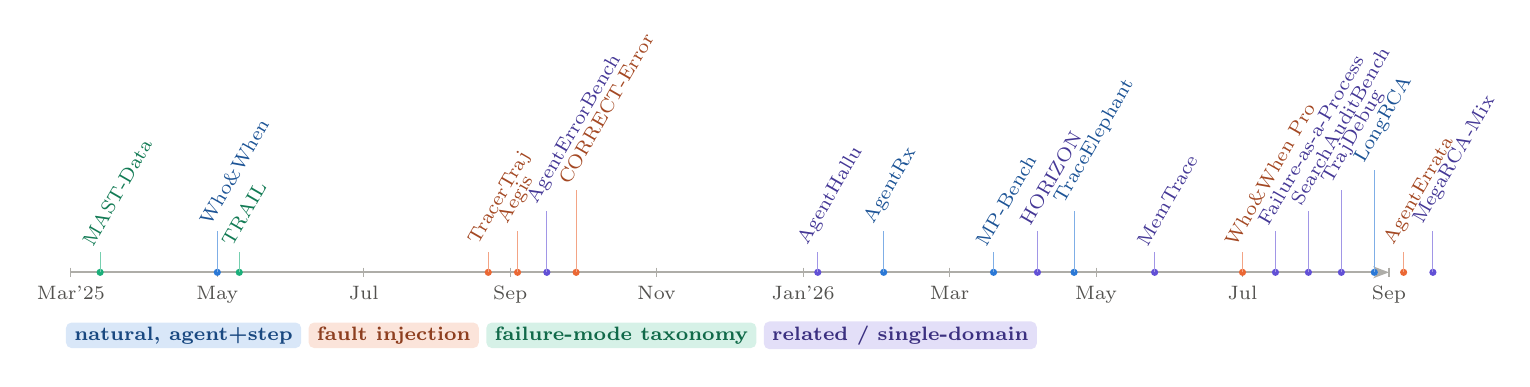
\begin{tikzpicture}[x=0.93cm,y=1cm,font=\scriptsize]
% timeline axis: Mar 2025 .. Oct 2026 -> 0 .. 17.6 cm (1 cm per month)
\def\tl{17.6}
\draw[-{Stealth[length=2mm]},rule!80!black,line width=0.6pt] (0,0) -- (\tl+0.4,0);
\foreach \m/\l in {0/Mar'25,2/May,4/Jul,6/Sep,8/Nov,10/Jan'26,12/Mar,14/May,16/Jul,18/Sep}{
  \draw[rule!80!black] (\m,0.06) -- (\m,-0.06); \node[below,color=ink2] at (\m,-0.05){\l};}
% events: month offset / level / color / label
\foreach \m/\lev/\c/\l in {
  0.4/1/s3/MAST-Data, 2.0/2/s1/Who\&When, 2.3/1/s3/TRAIL, 5.7/1/s2/TracerTraj, 6.1/2/s2/Aegis, 6.5/3/s7/AgentErrorBench, 6.9/4/s2/CORRECT-Error,
  10.2/1/s7/AgentHallu, 11.1/2/s1/AgentRx, 12.6/1/s1/MP-Bench, 13.2/2/s7/HORIZON, 13.7/3/s1/TraceElephant, 14.8/1/s7/MemTrace,
  16.0/1/s2/Who\&When Pro, 16.45/2/s7/Failure-as-a-Process, 16.9/3/s7/SearchAuditBench, 17.35/4/s7/TrajDebug, 17.8/5/s1/LongRCA,
  18.2/1/s2/AgentErrata, 18.6/2/s7/MegaRCA-Mix}{
  \fill[\c] (\m,0) circle (1.3pt);
  \draw[\c!60,line width=0.4pt] (\m,0) -- (\m,0.26*\lev);
  \node[anchor=south west,rotate=60,inner sep=1pt,text=\c!70!black] at (\m-0.08,0.26*\lev){\l};}
\node[anchor=north west,text=ink2] at (-0.2,-0.5){\chip{s1}{natural, agent+step}\ \chip{s2}{fault injection}\ \chip{s3}{failure-mode taxonomy}\ \chip{s7}{related / single-domain}};
\end{tikzpicture}
\vspace{-2pt}
\caption{Release timeline (month of the first arXiv version, approximate). Failure-attribution datasets appeared only after Who\&When (May 2025) and accelerated in 2026, moving from a few hundred hand-labelled logs to $10^4$ injected failures and to long-horizon, full-trace settings.}
\label{fig:timeline}
\end{figure}

\begin{table}[h]
\centering\scriptsize
\setlength{\tabcolsep}{2.5pt}
\begin{tabularx}{\linewidth}{@{}l l l l >{\RaggedRight\hsize=0.95\hsize}X r r >{\RaggedRight\hsize=1.05\hsize}X l@{}}\toprule
Dataset & Venue & Failures & System & Labels & \#failed & med.\ steps & Source frameworks / benchmarks & Access\\\midrule
\multicolumn{9}{@{}l}{\textbf{1\ \ Core MAS failure attribution (agent + decisive step)}}\\
Who\&When & ICML'25 & natural & MAS & agent, step, reason & 184 & 10 & CaptainAgent, Magentic-One / GAIA, AssistantBench & \okbadge\\
TraceElephant & ACL'26 & natural & MAS & agent, step, reason (full trace) & 220 & 21 & CaptainAgent, Magentic-One, SWE-Agent / GAIA, AB, SWE-bench & \okbadge\\
MP-Bench & ICML'26 & natural & MAS & agent, step sets (3 annotators) & 289 & -- & Who\&When logs + new runs & \okbadge\\
Who\&When Pro & ICML'26 & injected & MAS+single & agent, step, mode & 12\,326 & 4 & 15 frameworks / 26 benchmarks, text+image+video & \okbadge\\
LongRCA & arXiv'26 & natural & MAS & role, earliest root step & 1\,140 & 145 & 5 domains (TravelPlanner, WebArena, \dots) & \okbadge\\
AgentRx & EMNLP'26 & natural & MAS+single & step, 9-cat.\ taxonomy, events & 115 (73 public) & 33 & $\tau$-bench, Flash, Magentic-One & \gatedbadge\ \partialbadge\\
\midrule
\multicolumn{9}{@{}l}{\textbf{2\ \ Large injected-fault datasets (training attributors)}}\\
TracerTraj & ICLR'26 & injected & MAS & agent, step, reason & 3\,998 & 10 & MetaGPT-style, math, agentic & \okbadge\\
Aegis & ICLR'26 & injected & MAS & agent, 14 modes & 9\,533 & 10 & 6 MAS / GSM8K, MATH, HumanEval, MMLU, SciBench, GAIA & \okbadge\\
CORRECT-Error & ICML'26 & injected & MAS & agent, step & 2\,226 & 10 & Magentic-style / 7 QA+math benchmarks & \okbadge\\
AgentErrata & arXiv'26 & injected & MAS & agent, step, category & 303 & -- & Magentic-One / GAIA & \nobadge\\
\midrule
\multicolumn{9}{@{}l}{\textbf{3\ \ Failure-mode taxonomies (mostly no step label)}}\\
MAST-Data & NeurIPS'25 & natural & MAS & 14 modes (LLM judge; 21 human) & 1\,642 & 6 & 7 MAS / 8 benchmarks / 5 LLMs & \okbadge\\
TRAIL & arXiv'25 & natural & single+MAS & span-level errors, 3-level taxonomy, impact & 148 & 20 & smolagents / GAIA, SWE-bench & \okbadge\\
\midrule
\multicolumn{9}{@{}l}{\textbf{4\ \ Related trajectory-debugging datasets}}\\
AgentErrorBench / Traj2k & ICML'26 & natural & single & critical step, module + 17 types & 200 (Traj2k n/a) & 30 & ALFWorld, GAIA, WebShop & \okbadge\\
SearchAuditBench & arXiv'26 & natural & single & critical step, 6 root causes, repair rubric & 1\,243 & 43 & deep-search agents & \okbadge\\
Failure as a Process & arXiv'26 & natural & single & $t_{err}/t_{lock}/t_{obs}$, 9 triggers (annotations only) & 1\,184 (of 1\,794) & 22.5$^\ddagger$
 & Terminal-Bench CLI coding agents & \partialbadge\\
TrajErrBench & EMNLP'26 & natural & single & critical step, 20-type taxonomy & 486 & 29
 & $\tau^2$-Bench, SWE-Bench Pro & \okbadge\\
AgentHallu & arXiv'26 & natural & single(+MAS) & hallucination step, 5 cat./14 sub & 443 (of 693) & 6 & 7 frameworks / 8 benchmarks & \okbadge\\
MemTrace & arXiv'26 & natural & memory system & faulty memory op, 4 error types & 160 & 496$^\dagger$ & RAG, Mem0, EverMemOS, long-context & \okbadge\\
HORIZON & arXiv'26 & natural & single & mode (LLM judge); step on 294 & 2\,498 & 12 & OS, web, embodied, database & \partialbadge\\
MegaRCA-Mix & arXiv'26 & natural & single (Claude Code) & edge, fault side, 41 modes & 50 & -- & Harbor Index (GAIA, SWE-bench, HLE, \dots) & \nobadge\\
\bottomrule
\end{tabularx}
\caption{Overview. ``\#failed'' = labelled failed trajectories available (paper figure where the release differs; see each section). ``med.\ steps'' computed from the downloaded data. $^\dagger$MemTrace steps are memory operations in the dependency slice of the failed answer. $^\ddagger$Failure-as-a-Process: all 1\,794 runs, from the released annotations (trajectory text not released).}
\label{tab:overview}
\end{table}

\begin{figure}[htbp]
\centering
\begin{minipage}[t]{0.48\linewidth}\centering
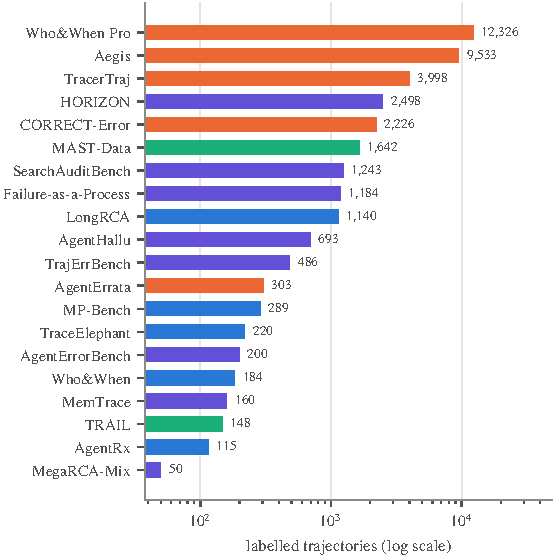
\includegraphics[width=\linewidth]{assets/figures/fig_sizes.pdf}
\captionof{figure}{Labelled failed trajectories per dataset (log scale). Injected-fault datasets (orange) are 1--2 orders of magnitude larger than human-labelled natural ones (blue).}\label{fig:sizes}
\end{minipage}\hfill
\begin{minipage}[t]{0.50\linewidth}\centering
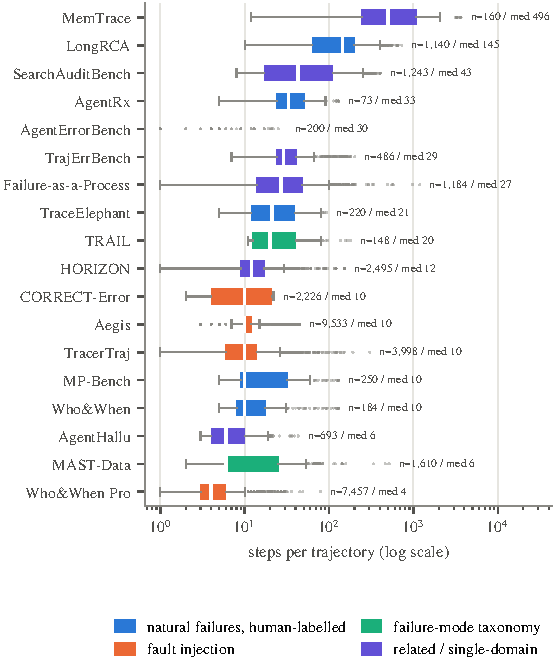
\includegraphics[width=\linewidth]{assets/figures/fig_steps.pdf}
\captionof{figure}{Steps per trajectory, computed from the downloaded data. Most benchmarks live in the 5--30 step range; LongRCA and MemTrace are the long-horizon outliers.}\label{fig:steps}
\end{minipage}
\end{figure}

\begin{figure}[htbp]
\centering
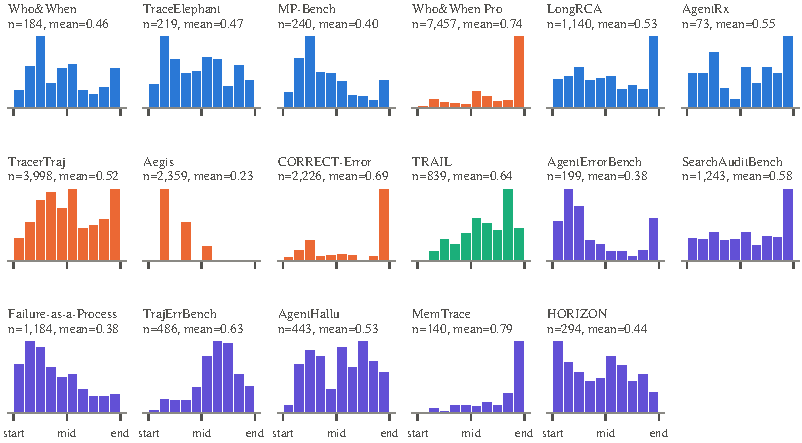
\includegraphics[width=0.92\linewidth]{assets/figures/fig_errpos.pdf}
\caption{Where the labelled error step sits inside the trajectory (relative position $t^\star/T$, 10 bins). Natural-failure benchmarks spread errors across the whole run with a spike at the end (the final wrong answer is often the labelled step); some injected datasets inject preferentially at the start (TracerTraj) or at the very end (Who\&When Pro, CORRECT-Error) --- a distribution shift to keep in mind when training on them.}
\label{fig:errpos}
\end{figure}


\section{Core MAS failure-attribution benchmarks (agent + decisive step)}\label{sec:g1}
\inputsec{who_and_when}
\inputsec{traceelephant}
\inputsec{mp_bench}
\inputsec{who_and_when_pro}
\inputsec{longrca}
\inputsec{agentrx}

\section{Large injected-fault datasets (mainly for training attributors)}\label{sec:g2}
\inputsec{tracertraj}
\inputsec{aegis}
\inputsec{correct_error}
\inputsec{agenterrata}

\section{Failure-taxonomy datasets (failure-mode labels)}\label{sec:g3}
\inputsec{mast_data}
\inputsec{trail}

\section{Related trajectory-debugging datasets}\label{sec:g4}
\inputsec{agenterrorbench}
\inputsec{searchauditbench}
\inputsec{failure_as_process}
\inputsec{trajerrbench}
\inputsec{agenthallu}
\inputsec{memtrace}
\inputsec{horizon}
\inputsec{megarca_mix}

\section{Cross-cutting observations and recommendations}\label{sec:reco}

\begin{multicols}{2}
\paragraph{No two datasets agree on what a ``step'' is} Who\&When counts every message, including orchestrator thoughts and the human question; TraceElephant counts trace events including tool I/O; TRAIL uses OpenTelemetry spans; MemTrace uses memory operations; AgentRx indexes 1-based from the system message; TracerTraj mixes 0- and 1-based indices across domains. Any evaluation that pools datasets must normalise the indexing explicitly---the normalised examples in \code{notes/*\_example\_norm.json} keep the dataset's own numbering for this reason.

\paragraph{Agent naming is a hidden evaluation knob} Agent-level accuracy is exact string match, yet names are inconsistent inside datasets (\code{WebSurfer}/\code{Websurfer} in Who\&When, \code{Assistant}/\code{assistant} in AgentRx) and generic in others (TracerTraj's agentic split labels every step \code{assistant}, making agent-level accuracy trivial). Normalise case and collapse orchestrator variants before scoring.

\paragraph{Single root cause is a modelling choice} Who\&When, TracerTraj, CORRECT-Error and LongRCA store one decisive step. MP-Bench shows three experts agree on a single failure-inducing step in only 16\% of logs; AgentRx records multiple failure \emph{events} plus a root cause (root $\ne$ first failure in 27\% of public records); TRAIL labels every error span; MegaRCA scores a \emph{set} of (edge, fault, mode) triples with F1. For evaluation, report a window-tolerant step metric alongside exact match, and prefer MP-Bench or AgentRx when the method produces several candidates.

\paragraph{Natural versus injected} Human-labelled natural failures (Who\&When, TraceElephant, MP-Bench, LongRCA, AgentRx, TRAIL; $\approx$2\,k trajectories in total) are the only trustworthy \emph{test} sets. Injected datasets (Who\&When Pro, Aegis, TracerTraj, CORRECT-Error; $\approx$28\,k) are the only practical \emph{training} sets, but their error-position and error-type distributions are skewed (Fig.~\ref{fig:errpos}): Aegis is near-uniform over 14 modes by design, Who\&When Pro and CORRECT-Error concentrate labels at the last step, TracerTraj at the first steps. Evaluate cross-distribution.

\paragraph{Observation level matters} Output-only logs (Who\&When, MAST-Data) hide tool inputs, screenshots and environment state. TraceElephant reports up to +76\% relative attribution accuracy from full traces and ships reproducible environments for counterfactual replay; LongRCA keeps $\approx$180\,k characters per trajectory; MemTrace stores complete execution graphs (up to 500\,MB per file). Decide early whether the attributor is meant to work from logs or from live replay.

\paragraph{Label provenance} Only Who\&When, TraceElephant, MP-Bench, LongRCA, AgentRx, TRAIL, AgentHallu, MemTrace, Failure-as-a-Process, SearchAuditBench and MegaRCA-Mix are human-labelled. MAST-Data (14 modes) and HORIZON are labelled by an LLM judge (MAST validated on 21 traces, $\kappa\approx0.88$ reported in the paper); Aegis and CORRECT-Error labels are correct by construction but describe injected, not observed, errors.

\paragraph{Recommended protocol}
\begin{enumerate}[leftmargin=1.2em]
\item \textbf{Standard evaluation}: Who\&When (both subsets), TraceElephant (full-trace) and MP-Bench (multi-annotator); report agent accuracy, exact-step accuracy, and step accuracy within $\pm k$ steps.
\item \textbf{Scale / long traces}: add Who\&When Pro (26 benchmarks, 3 modalities) and LongRCA (median 145 steps; use LongRCA-Mini for screening).
\item \textbf{Training}: TracerTraj and Aegis (both with train/val/test splits); CORRECT-Error as a third, Magentic-style source. Hold out one natural dataset for cross-distribution testing.
\item \textbf{Diagnosis beyond ``who/when''}: MAST-Data for failure-mode classification, TRAIL for span-level multi-error localisation, AgentRx for taxonomy + root cause on tool-calling agents.
\item \textbf{Generalisation checks}: AgentErrorBench (embodied/web), SearchAuditBench (deep search), Failure-as-a-Process (CLI coding), AgentHallu (hallucination), MemTrace (memory).
\item \textbf{Licensing}: several datasets carry no explicit license (Who\&When, LongRCA, TracerTraj, HORIZON); AgentRx and HORIZON-tasks are gated; MegaRCA-Mix and AgentErrata (and parts of AgentRx) are not public as of 16 Oct 2026. Verify before redistribution.
\end{enumerate}
\end{multicols}

\section{Future work: counterfactual outcome prediction for agent trajectories}\label{sec:future}

\begin{multicols}{2}
\paragraph{Motivation} Every attribution dataset in this survey defines the decisive step counterfactually---``the step that, had it been correct, would have let the run succeed''---yet none of them tests that claim. Labels come from a human or an LLM reading a single observed continuation, and the data show how fragile such labels are: three experts agree on one failure-inducing step in only 16\% of MP-Bench logs (\S\ref{sec:reco}), and our own re-analysis of the released files (\code{scripts/explore/}) adds two more observations: on the 86 tasks that Who\&When and TraceElephant both ran in the same system family, the blamed agent coincides in only 18, and 240 of 685 LongRCA TravelPlanner reasons cite an external verifier verdict that is not in the trajectory at all. The datasets that \emph{do} intervene use replay only as an annotation or data-generation tool: TraceElephant re-executes from a candidate step to confirm a label \citep{traceelephant2026}, AgentDebug fixes a step and reruns to validate a diagnosis \citep{agentdebug2026}, and Aegis, Who\&When~Pro and TracerTraj inject faults into successful runs and keep the ones that fail \citep{aegis2026,whowhenpro2026,agentracer2026}. Aegis reports that an injection flips the outcome in 34.1\% (DyLAN) to 76.5\% (Debate) of attempts, i.e.\ the same perturbation has very different effects depending on the system---but nobody has tried to \emph{predict} that effect. We propose to make the intervention effect itself the prediction target, in the spirit of perturbation-response prediction in single-cell biology, where a model predicts the expression change caused by a gene knock-out rather than the unperturbed state \citep{roohani2024gears}. The two motivating questions are
\begin{itemize}[leftmargin=1.1em,itemsep=1pt]
\item[\textbf{Q1}] If one step of a \emph{failed} trajectory is changed and the run is resumed from that point, does it succeed?
\item[\textbf{Q2}] If an error is injected into one step of a \emph{successful} trajectory and the run is resumed from that point, does it fail?
\end{itemize}
Both are ambiguous as stated (``does it succeed'' under a stochastic system is a probability; ``changed'' needs a vocabulary; ``resumed'' needs a replay semantics). The formulation below fixes each ambiguity.
\end{multicols}

\subsection{Problem formulation}\label{sec:future:formal}

\begin{multicols}{2}
\paragraph{Setting}
\begin{definition}[Task, environment, grader]\label{def:env}
A \emph{task} $x\in\mathcal X$ comes with a sandboxed \emph{environment} $E_x=(\mathcal Z, z_0, f, \omega)$---state space, initial state, transition $z_t=f(z_{t-1},a_t)$ and observation map $o_t=\omega(z_t)$---and a \emph{grader} $g_x:\mathcal Y\to\{0,1\}$ on final outputs. $f$, $\omega$ and $g_x$ are deterministic functions.
\end{definition}

\begin{definition}[Agentic system and trajectory]\label{def:traj}
An \emph{agentic system} $\pi$ consists of a finite agent set $\mathcal A$, a scheduler $\sigma$ and per-agent policies $\pi_\alpha$. At step $t$ the scheduler picks $\alpha_t=\sigma(h_{t-1})$ and the agent samples an action $a_t\sim\pi_{\alpha_t}(\cdot\mid x,h_{t-1})$ (an LLM call: message, tool call or code). The environment answers with $o_t$. A \emph{step} is $s_t=(\alpha_t,a_t,o_t)$, a \emph{prefix} is $h_t=(s_1,\dots,s_t)$ (with $h_0=\varnothing$), and a \emph{trajectory} $\tau=h_T$ ends when the system emits a final output $y(\tau)\in\mathcal Y$ or exhausts a budget $B$ (steps, tokens or wall-clock); exhaustion counts as $y=\bot$ with $g_x(\bot)=0$. The \emph{outcome} is $Y(\tau)=g_x(y(\tau))\in\{0,1\}$.
\end{definition}
All randomness lives in the policies (sampling at temperature $>0$); the environment and grader are fixed. This is the regime of every dataset in \S\ref{sec:g1}--\ref{sec:g4} except the live-web ones, which violate Assumption~\ref{as:replay} below.

\begin{definition}[Continuation law and value]\label{def:value}
Let $P_\pi(\cdot\mid x,h_t)$ denote the distribution over complete trajectories obtained by \emph{resuming} $\pi$ from prefix $h_t$: the environment is restored to $z_t$, the conversation state of every agent is restored to what it was after $h_t$, and the remaining budget is $B$ minus what $h_t$ consumed. The \emph{value} of a prefix is
\[
V(h_t)\;=\;\mathbb E_{\tau'\sim P_\pi(\cdot\mid x,h_t)}\big[Y(\tau')\big]\in[0,1].
\]
\end{definition}

\begin{assumption}[Replayability]\label{as:replay}
For every prefix $h_t$ the state $z_t$ can be reconstructed, either from a snapshot or by deterministically replaying $a_1,\dots,a_t$ from $z_0$. The latter is \emph{verified} by a replay check: the recomputed observations must equal the recorded $o_1,\dots,o_t$ byte for byte. Prefixes that fail the check are excluded.
\end{assumption}

\begin{assumption}[Fixed system]\label{as:system}
Model versions, prompts, tools, temperature and budget $B$ are pinned for the whole study; random seeds are \emph{not} fixed, so that $P_\pi(\cdot\mid x,h_t)$ reflects the system's own run-to-run variability (which is large: \S\ref{sec:reco}, point on run-specific root causes).
\end{assumption}

\paragraph{Interventions}
\begin{definition}[Intervention]\label{def:interv}
An \emph{intervention} is a pair $\iota=(t,\phi)$ of a target step index $t\in\{1,\dots,T\}$ and a \emph{step editor} $\phi$. Two editor classes are distinguished by what the environment recomputes:
\begin{itemize}[leftmargin=1.1em,itemsep=1pt]
\item \emph{action-level}: $\phi$ replaces the action, $a_t'=\phi(x,h_{t-1},s_t)$, and the observation is recomputed, $o_t'=\omega(f(z_{t-1},a_t'))$; the agent identity is kept, $\alpha_t'=\alpha_t$;
\item \emph{observation-level}: $\phi$ keeps $a_t$ and replaces $o_t$ by $o_t'=\phi(x,h_{t-1},s_t)$, simulating a corrupted tool result or environment reply; the environment state is left at $f(z_{t-1},a_t)$.
\end{itemize}
The \emph{intervened prefix} is $h_t^{\iota}=(s_1,\dots,s_{t-1},s_t')$ with $s_t'=(\alpha_t,a_t',o_t')$. Steps after $t$ are \textbf{never copied} from the observed trajectory: the continuation is regenerated from $h_t^{\iota}$ under Definition~\ref{def:value}. This is the $\mathrm{do}(s_t:=s_t')$ semantics; ``editing step $t$ and keeping the rest'' is not an intervention in this sense.
\end{definition}

\begin{definition}[Repair and corruption vocabularies]\label{def:vocab}
A \emph{repair} $\phi\in\Phi^{+}$ is an editor intended to make step $t$ correct for $x$. Two privilege levels are recorded: an \emph{oracle repair} may use the ground truth and the recorded continuation; an \emph{unprivileged repair} may use only $(x,h_{t-1},s_t)$ and a free-text diagnosis (e.g.\ \code{mistake\_reason}). A \emph{corruption} $\phi\in\Phi^{-}$ is an editor drawn from an error-mode taxonomy $\mathcal M$ (the 14 Aegis modes or the Who\&When~Pro families, \S\ref{sec:g2}) at a severity level $\ell\in\{1,2,3\}$; it must produce a step that the system accepts as well-formed. Every editor is applied by a fixed procedure (a prompted model plus human check), and the resulting $s_t'$ is stored, so that the intervention is a concrete, inspectable object rather than a description.
\end{definition}

\paragraph{Estimands}
\begin{definition}[Intervention effect]\label{def:effect}
For a prefix $h_t$ and intervention $\iota=(t,\phi)$,
\[
\Delta(h_t,\iota)\;=\;V(h_t^{\iota})-V(h_t)\;\in[-1,1].
\]
\end{definition}
Both arms share $x$, $h_{t-1}$ and $\pi$ and differ only in $s_t$, so $\Delta$ is an average treatment effect with assignment by design; no adjustment for confounders is needed \citep{shalit2017ite}. The two motivating questions become:

\begin{task}[Q1, repair effect]\label{task:q1}
Given an observed trajectory $\tau$ with $Y(\tau)=0$, a step index $t$ and a repair $\iota=(t,\phi)$, $\phi\in\Phi^{+}$, predict $\Delta^{+}(\tau,\iota)=\Delta(h_t,\iota)$.
\end{task}
\begin{task}[Q2, injection effect]\label{task:q2}
Given an observed trajectory $\tau$ with $Y(\tau)=1$, a step index $t$ and a corruption $\iota=(t,\phi)$, $\phi\in\Phi^{-}$, predict $\Delta^{-}(\tau,\iota)=-\Delta(h_t,\iota)=V(h_t)-V(h_t^{\iota})$.
\end{task}
Note that the comparison is between the \emph{two rerun arms}, not between the rerun and the single observed bit $Y(\tau)$: a failed run may have $V(h_t)>0$ and a successful run $V(h_t)<1$ under Assumption~\ref{as:system}. ``Does the repaired run succeed?'' is therefore read as $V(h_t^{\iota})$, and ``does the repair \emph{matter}?'' as $\Delta^{+}$; both are reported.

\begin{definition}[Monte-Carlo labels]\label{def:labels}
Each arm is rerun $n$ times independently, giving $\hat V_n(h)=\frac1n\sum_{i=1}^{n}Y(\tau'^{(i)})$ and $\hat\Delta_n=\hat V_n(h_t^{\iota})-\hat V_n(h_t)$. A label is the triple $(\hat V_n(h_t),\hat V_n(h_t^{\iota}),n)$ with exact binomial (Clopper--Pearson) intervals; $\operatorname{se}(\hat\Delta_n)\le 1/\sqrt{2n}$, i.e.\ $0.25$ at $n=8$. Allocation is sequential: arms whose first $n_0=4$ replicates are unanimous stop; disagreeing arms continue to $n=16$.
\end{definition}

\paragraph{Prediction tasks} A \emph{predictor} $F$ outputs $\hat\Delta\in[-1,1]$ (or the pair $\hat V(h_t),\hat V(h_t^{\iota})$) from an input $u$ and is \textbf{not allowed to execute the environment} (otherwise Definition~\ref{def:labels} is the trivial solution; a budgeted variant allowing $b\ll n$ rollouts is a separate track). Three observability regimes are defined by what $u$ contains:
\begin{itemize}[leftmargin=1.1em,itemsep=1pt]
\item[R0] $(x,h_{t-1},s_t,s_t')$ and a description of $\pi$---the \emph{prospective} regime, the only one available online;
\item[R1] R0 plus the recorded continuation $s_{t+1},\dots,s_T$ and $Y(\tau)$---the \emph{post-mortem} regime of failure attribution;
\item[R2] R1 plus full traces (tool I/O, screenshots, prompts), as in TraceElephant.
\end{itemize}
The three regimes are evaluated separately; R1$-$R0 measures how much the observed future tells about the counterfactual one.

\paragraph{Derived quantities} The formulation subsumes the tasks of this survey and two new ones. Fix an effect threshold $\theta\in(0,1)$ (we use $\theta=0.25$, the resolution of $n=8$).
\begin{definition}[Decisive step and responsible agent]\label{def:decisive}
For a failed $\tau$ and a repair vocabulary $\Phi^{+}$,
\[
t^\star(\tau)=\min\Big\{t:\ \max_{\phi\in\Phi^{+}}\Delta\big(h_t,(t,\phi)\big)\ge\theta\Big\},\qquad \alpha^\star(\tau)=\alpha_{t^\star}.
\]
If the set is empty, $\tau$ has \emph{no decisive step} under $\Phi^{+}$ (several independent errors, or a cause outside the trajectory). $t^\star$ is ``earliest effective'', matching the Who\&When convention; the \emph{most} effective step $\arg\max_t\max_\phi\Delta$ is reported alongside. A repair is \emph{sufficient} if $V(h_t^{\iota})\ge1-\theta$, \emph{necessary-only} if $\Delta\ge\theta$ but $V(h_t^{\iota})<1-\theta$.
\end{definition}
\begin{definition}[Lock-in time]\label{def:lock}
For a failed $\tau$,
\[
t_{\mathrm{lock}}(\tau)=\min\Big\{t:\ \max_{t'\ge t,\ \phi\in\Phi^{+}}\Delta\big(h_{t'},(t',\phi)\big)<\theta\Big\},
\]
the step after which no single-step repair recovers the run; the Failure-as-a-Process $t_{\mathrm{lock}}$ (\S\ref{sec:g4}) is the human estimate of this quantity.
\end{definition}
\begin{definition}[Robustness profile]\label{def:robust}
For a system $\pi$, corruption mode $m\in\mathcal M$ and relative position $\rho=t/T$, $R_\pi(m,\rho)=1-\mathbb E\big[\Delta^{-}\mid m,\rho\big]$ over successful trajectories; $R_\pi$ close to 1 means the system absorbs that error at that position. Aegis's per-framework injection success rates are marginal estimates of $1-R_\pi$.
\end{definition}

\paragraph{Metrics} For a test set of labelled triples: (i)~mean absolute error and Brier score of $\hat\Delta$ against $\hat\Delta_n$, reported together with the \emph{noise floor} $\mathbb E[\operatorname{var}(\hat\Delta_n)]$ that even a perfect predictor cannot beat; (ii)~AUROC of $\hat\Delta$ for the event $\{\hat\Delta_n\ge\theta\}$; (iii)~expected calibration error of $\hat\Delta$; (iv)~within-trajectory Spearman correlation between predicted and measured effects over the candidate steps of the same trajectory, which is the quantity that decides attribution; (v)~attribution accuracy of $\hat t^\star$ (Definition~\ref{def:decisive} computed from $\hat\Delta$) against $t^\star$ computed from the Monte-Carlo labels, exact and within $\pm k$ steps.

\paragraph{Relation to the biology analogy} Prefix $h_{t-1}$ plays the role of the cell state, $\iota$ of the perturbation and $\Delta$ of the response; generalisation to \emph{unseen} perturbations corresponds to held-out editor types and held-out steps. Two differences matter: the perturbation space here is open-ended (hence the fixed vocabularies of Definition~\ref{def:vocab}), and effects compound sequentially, so the same editor has position-dependent effects (hence $\rho$ in Definition~\ref{def:robust}).
\end{multicols}

\begin{center}
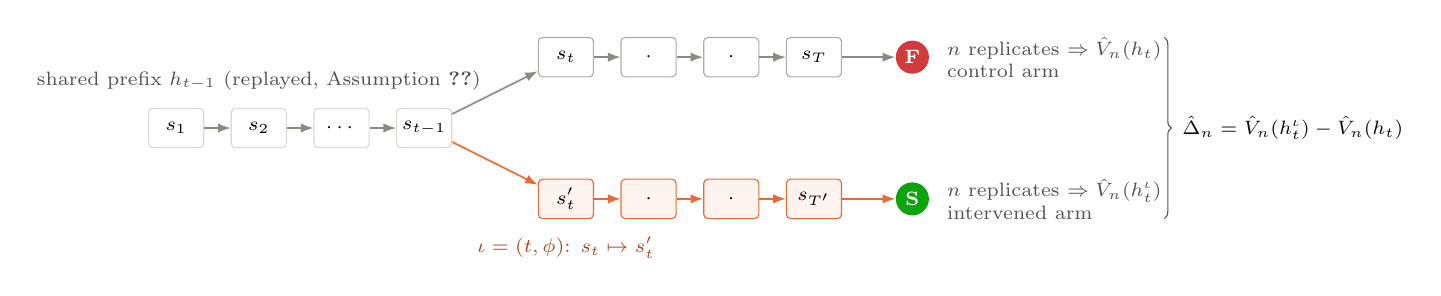
\begin{tikzpicture}[x=1cm,y=1cm,font=\scriptsize,
  st/.style={draw=rule,fill=white,rounded corners=1.5pt,minimum width=7mm,minimum height=5mm,inner sep=1pt},
  ctl/.style={st,draw=ink3!70},
  trt/.style={st,draw=s2,fill=s2!8},
  outc/.style={circle,minimum size=4.2mm,inner sep=0pt,font=\scriptsize\bfseries,text=white},
  ar/.style={-{Latex[length=1.6mm]},draw=ink3,semithick}]
  \foreach \i/\n in {1/$s_1$,2/$s_2$,3/$\cdots$,4/$s_{t-1}$} {\node[st] (p\i) at (\i*1.05,0) {\n};}
  \foreach \i in {1,2,3} {\pgfmathtruncatemacro{\j}{\i+1}\draw[ar] (p\i) -- (p\j);}
  \node[above=1mm of p2.north,anchor=south,text=ink2] {shared prefix $h_{t-1}$ (replayed, Assumption~\ref{as:replay})};
  \node[ctl] (c0) at (6,0.9) {$s_t$};
  \foreach \i in {1,2} {\node[ctl] (c\i) at (6+\i*1.05,0.9) {$\cdot$};}
  \node[ctl] (cT) at (9.15,0.9) {$s_{T}$};
  \draw[ar] (p4) -- (c0); \draw[ar] (c0)--(c1); \draw[ar] (c1)--(c2); \draw[ar] (c2)--(cT);
  \node[outc,fill=critical] (cf) at (10.4,0.9) {F};
  \draw[ar] (cT)--(cf);
  \node[right=1mm of cf,text=ink2,align=left] {$n$ replicates $\Rightarrow \hat V_n(h_t)$\\control arm};
  \node[trt] (t0) at (6,-0.9) {$s_t'$};
  \foreach \i in {1,2} {\node[trt] (t\i) at (6+\i*1.05,-0.9) {$\cdot$};}
  \node[trt] (tT) at (9.15,-0.9) {$s_{T'}$};
  \draw[ar,draw=s2] (p4) -- (t0); \draw[ar,draw=s2] (t0)--(t1); \draw[ar,draw=s2] (t1)--(t2); \draw[ar,draw=s2] (t2)--(tT);
  \node[outc,fill=good] (ts) at (10.4,-0.9) {S};
  \draw[ar,draw=s2] (tT)--(ts);
  \node[right=1mm of ts,text=ink2,align=left] {$n$ replicates $\Rightarrow \hat V_n(h_t^{\iota})$\\intervened arm};
  \node[below=1mm of t0.south,text=s2!70!black] {$\iota=(t,\phi)$: $s_t\mapsto s_t'$};
  \draw[decorate,decoration={brace,amplitude=2.5pt},ink2] (13.6,1.15) -- (13.6,-1.15) node[midway,right=3pt,text=ink] {$\hat\Delta_n=\hat V_n(h_t^{\iota})-\hat V_n(h_t)$};
\end{tikzpicture}
\captionof{figure}{Counterfactual outcome prediction (Definitions~\ref{def:interv}--\ref{def:labels}). From a shared, replayed prefix, the control arm continues with the recorded step $s_t$ and the intervened arm with $s_t'$; steps after $t$ are regenerated in both arms, $n$ times each, under the system's own stochasticity. The prediction target is the difference in success frequency, not the outcome of either arm.}\label{fig:cfo}
\end{center}

\begin{multicols}{2}
\paragraph{Why it is not outcome prediction} Predicting $V(h_t)$ is what process reward models and early-failure predictors do \citep{lightman2023prm}. The objection that ``a correct step $t$ does not guarantee later steps are correct, and a wrong step $t$ may be corrected later'' applies to both questions, but it affects them differently. (i)~\emph{Confounding.} A value model learns from observed runs that sloppy prefixes come from runs that fail---but also from hard tasks, weak models and bad configurations. It can score well by recognising a failing run without learning that step $t$ \emph{causes} the failure; the paired design of Definition~\ref{def:effect} removes this by construction. (ii)~\emph{Variance.} Task difficulty and prefix quality are held fixed across arms, so $\Delta$ is estimated with lower variance than an absolute outcome, exactly as in a paired experiment. (iii)~\emph{The attenuation is the signal.} $\Delta^{+}$ is attenuated by the probability of independent downstream failures (MP-Bench annotators flag several scattered errors per run), and $\Delta^{-}$ is attenuated by the system's recovery capacity (Aegis's per-framework flip rates). A decisive step is precisely one whose repair effect survives the rest of the run; a robust system is one in which injection effects are small. Outcome prediction cannot separate ``the step was wrong'' from ``the step was wrong and nothing downstream absorbed it''; $\Delta$ measures the second thing directly. The two coincide only in a deterministic system where the intervention makes the remainder identical to a known successful run.

\paragraph{Benchmark construction} The limiting resource is Assumption~\ref{as:replay}; of the 20 datasets only TraceElephant ships environments, and live-web tasks (GAIA, AssistantBench, WebArena on public sites) drift between runs. We therefore propose sandboxed environments with deterministic graders, using the existing datasets as sources of prefixes and interventions:
\begin{itemize}[leftmargin=1.1em,itemsep=1pt]
\item \textbf{Environments}: SWE-Bench Verified (TraceElephant's SWE-Agent traces and released agent code; snapshot = container state), $\tau^2$-bench and TravelPlanner (tool calling with a simulated user and a rule-based checker; snapshot = database state), ALFWorld/WebShop (as in AgentErrorBench), and the Who\&When~Pro harness for multi-agent runs over offline benchmarks.
\item \textbf{Prefixes}: the 220 TraceElephant failures and their decisive steps for Task~\ref{task:q1}; fresh successful runs in the same environments for Task~\ref{task:q2}; for every prefix also 3--5 \emph{control} steps chosen uniformly at random, so that the label set contains effects near zero.
\item \textbf{Editors}: repairs from MP-Bench's \code{ideal\_action}, SearchAuditBench's repair directives and the \code{mistake\_reason} text of Who\&When/TraceElephant, turned into a concrete $s_t'$ by a strong model and checked by a human (oracle and unprivileged variants, Definition~\ref{def:vocab}); corruptions from the Aegis modes and the Who\&When~Pro taxonomy at three severities and at several relative positions $\rho$.
\item \textbf{Replicates}: Definition~\ref{def:labels}, $n_0=4$ to $n=16$. A by-product is a replicate-based $V(h_t)$ for every prefix, a far better outcome-prediction label than the single observed bit that PRM datasets use.
\item \textbf{Splits}: held-out tasks, held-out editor types and held-out systems, mirroring the cross-distribution evaluation recommended in \S\ref{sec:reco}; R0/R1/R2 are evaluated separately.
\end{itemize}
A first version with 200 prefixes $\times$ 4 interventions (1 labelled + 3 control steps) $\times$ 2 arms $\times$ 8 replicates is $\approx$13\,k partial reruns; because runs resume at step $t$, the average rerun is a fraction of a full trajectory, and the cost is in the low thousands of dollars at current API prices.

\paragraph{Models and baselines}
\begin{enumerate}[leftmargin=1.2em,itemsep=1pt]
\item \textbf{Priors}: relative position $\rho$ and corruption severity $\ell$ alone. These must be reported because late, severe injections always fail and single repairs rarely rescue long runs.
\item \textbf{Value-model difference}: a PRM-style model trained on $\hat V_n(h_t)$, scoring $\hat V(h_t^{\iota})-\hat V(h_t)$. This is the decisive baseline: if it matches the measured $\Delta$, the effect question reduces to outcome prediction and the contribution is the benchmark.
\item \textbf{LLM judge}: a prompted frontier model asked for $\hat\Delta$ in each regime R0--R2.
\item \textbf{Direct effect predictor}: a model trained on $(x,h_{t-1},s_t,s_t')$ against $\hat\Delta_n$ with a shared encoder for both arms, in the TARNet style \citep{shalit2017ite}; loss weighted by the label precision $1/\operatorname{var}(\hat\Delta_n)$.
\end{enumerate}

\paragraph{Hypotheses} \textbf{H1}: the annotated decisive step of TraceElephant has $\Delta^{+}\ge\theta$ in a minority of runs when repaired in isolation, i.e.\ current step labels are mostly necessary but not sufficient causes (Definition~\ref{def:decisive}). \textbf{H2}: the value-model difference correlates only weakly with measured $\Delta$, because the observational model absorbs task difficulty rather than step causality. \textbf{H3}: $R_\pi(m,\rho)$ decreases in $\rho$ and in severity with a system-specific rate, matching the Aegis flip rates. If H1 holds, the benchmark also delivers the first counterfactually validated attribution labels, which can be fed back to every dataset in \S\ref{sec:g1}.

\paragraph{Risks} Non-determinism makes single reruns meaningless (hence Definition~\ref{def:labels}); environments drift (hence Assumptions~\ref{as:replay}--\ref{as:system}); editors can be unrealistic (hence human-checked repairs and severity-graded corruptions); and some causes are not in the trajectory at all (LongRCA's evaluator verdicts), so a share of prefixes will have $\Delta\approx0$ for every editor---these are kept, not filtered, as they are the ``no decisive step'' cases of Definition~\ref{def:decisive} that MP-Bench and TraceElephant already contain.

\paragraph{Milestones} (1)~Validation study: repair the labelled step of every TraceElephant SWE-Agent trace with replicates and report the flip rate, a one-month effort that tests H1 on its own. (2)~Task~\ref{task:q2} benchmark in two sandboxed environments with graded corruptions. (3)~Task~\ref{task:q1} benchmark with human-checked repairs. (4)~Baselines 1--4 and the three generalisation splits. The novelty is not the replay machinery, which exists, but the shift from using it to \emph{produce} labels to treating the effect it measures as the thing to \emph{predict}.
\end{multicols}

\clearpage
\bibliographystyle{plainnat}\bibliography{bib/refs_merged}
\end{document}
